%%%%%%%% ICML 2026 EXAMPLE LATEX SUBMISSION FILE %%%%%%%%%%%%%%%%%

\documentclass{article}

% Recommended, but optional, packages for figures and better typesetting:
\usepackage{microtype}
\usepackage{graphicx}
\usepackage{subcaption}
\usepackage{booktabs} % for professional tables

% hyperref makes hyperlinks in the resulting PDF.
% If your build breaks (sometimes temporarily if a hyperlink spans a page)
% please comment out the following usepackage line and replace
% \usepackage{icml2026} with \usepackage[nohyperref]{icml2026} above.
\usepackage{hyperref}


% Attempt to make hyperref and algorithmic work together better:
\newcommand{\theHalgorithm}{\arabic{algorithm}}

% Use the following line for the initial blind version submitted for review:
\usepackage{icml2026}

% For preprint, use
% \usepackage[preprint]{icml2026}

% If accepted, instead use the following line for the camera-ready submission:
% \usepackage[accepted]{icml2026}

\usepackage{amsmath}
\usepackage{amssymb}
\usepackage{mathtools}
\usepackage{amsthm}


% if you use cleveref..
\usepackage[capitalize,noabbrev]{cleveref}

% ---- Packages ----
\usepackage{microtype}
\usepackage{graphicx}
\usepackage{subcaption}
\usepackage{booktabs}
\usepackage{multirow}
\usepackage{amsmath, amssymb, amsfonts}
\usepackage{mathtools}
\usepackage{bm}
\usepackage{algorithm}
\usepackage{algorithmic}
\usepackage{hyperref}
\usepackage{cleveref}
% \usepackage{enumitem}
\usepackage[inline, shortlabels]{enumitem}
\usepackage{xcolor}
\usepackage{amsthm}

% ---- Optional: TikZ for figures ----
\usepackage{tikz}
\usetikzlibrary{positioning, arrows.meta, calc}
\newcommand{\probP}{\text{I\kern-0.15em P}}

% --- Tickz
\usepackage{physics}
\usepackage{tikz}
\usetikzlibrary{arrows.meta,positioning,fit,calc}
\usepackage{amsmath}
\usepackage{mathdots}
% \usepackage{yhmath}
\usepackage{cancel}
\usepackage{color}
\usepackage{siunitx}
\usepackage{array}
\usepackage{stmaryrd}
\usepackage{multirow}
% \usepackage{amssymb}
\usepackage{gensymb}
\usepackage{tabularx}
\usepackage{extarrows}
\usepackage{booktabs}
\usetikzlibrary{fadings}
\usetikzlibrary{patterns}
\usetikzlibrary{shadows.blur}
\usetikzlibrary{shapes}

% ---- Math shortcuts ----
\newcommand{\E}{\mathbb{E}}
\newcommand{\R}{\mathbb{R}}
\newcommand{\I}{\mathbb{I}}

\usepackage{amssymb}
\usepackage{pifont}

\newcommand{\cmark}{\ding{51}}%
\newcommand{\xmark}{\ding{55}}%

\usepackage[english]{babel}
\addto\extrasenglish{  
    \def\figureautorefname{Figure}
    \def\tableautorefname{Table}
    \def\algorithmautorefname{Algorithm}
    \def\sectionautorefname{Section}
    \def\subsectionautorefname{Subsection}
    \def\proofoutlineautorefname{Proof Outline}
}

%%%%%%%%%%%%%%%%%%%%%%%%%%%%%%%%
% THEOREMS
%%%%%%%%%%%%%%%%%%%%%%%%%%%%%%%%
\theoremstyle{plain}
\newtheorem{theorem}{Theorem}[section]
\newtheorem{proposition}[theorem]{Proposition}
\newtheorem{lemma}[theorem]{Lemma}
\newtheorem{corollary}[theorem]{Corollary}
\theoremstyle{definition}
\newtheorem{definition}[theorem]{Definition}
\newtheorem{assumption}[theorem]{Assumption}
\theoremstyle{remark}
\newtheorem{remark}[theorem]{Remark}

% Todonotes is useful during development; simply uncomment the next line
%    and comment out the line below the next line to turn off comments
%\usepackage[disable,textsize=tiny]{todonotes}
\usepackage[textsize=tiny]{todonotes}

% The \icmltitle you define below is probably too long as a header.
% Therefore, a short form for the running title is supplied here:
\icmltitlerunning{Neuro-Symbolic Multi-Agent World Models}

\begin{document}

\twocolumn[
  \icmltitle{A Neuro-Symbolic Multi-Agent World Model Framework\\
    for Model-Based Multi-Agent Reinforcement Learning}

  % It is OKAY to include author information, even for blind submissions: the
  % style file will automatically remove it for you unless you've provided
  % the [accepted] option to the icml2026 package.

  % List of affiliations: The first argument should be a (short) identifier you
  % will use later to specify author affiliations Academic affiliations
  % should list Department, University, City, Region, Country Industry
  % affiliations should list Company, City, Region, Country

  % You can specify symbols, otherwise they are numbered in order. Ideally, you
  % should not use this facility. Affiliations will be numbered in order of
  % appearance and this is the preferred way.
  \icmlsetsymbol{equal}{*}

  \begin{icmlauthorlist}
    \icmlauthor{Julien Soulé}{equal,yyy}
    \icmlauthor{Georgios Bakirtzis}{equal,yyy,comp}
    \icmlauthor{Jean-Paul Jamont}{comp}
    \icmlauthor{Firstname4 Lastname4}{sch}
    \icmlauthor{Firstname5 Lastname5}{yyy}
    \icmlauthor{Firstname6 Lastname6}{sch,yyy,comp}
    \icmlauthor{Firstname7 Lastname7}{comp}
    %\icmlauthor{}{sch}
    \icmlauthor{Firstname8 Lastname8}{sch}
    \icmlauthor{Firstname8 Lastname8}{yyy,comp}
    %\icmlauthor{}{sch}
    %\icmlauthor{}{sch}
  \end{icmlauthorlist}

  \icmlaffiliation{yyy}{Department of XXX, University of YYY, Location, Country}
  \icmlaffiliation{comp}{Company Name, Location, Country}
  \icmlaffiliation{sch}{School of ZZZ, Institute of WWW, Location, Country}

  \icmlcorrespondingauthor{Julien Soulé}{julien.soule@hotmail.fr}
  \icmlcorrespondingauthor{Firstname2 Lastname2}{first2.last2@www.uk}

  % You may provide any keywords that you find helpful for describing your
  % paper; these are used to populate the "keywords" metadata in the PDF but
  % will not be shown in the document
  \icmlkeywords{Machine Learning, ICML}

  \vskip 0.3in
]

% this must go after the closing bracket ] following \twocolumn[ ...

% This command actually creates the footnote in the first column listing the
% affiliations and the copyright notice. The command takes one argument, which
% is text to display at the start of the footnote. The \icmlEqualContribution
% command is standard text for equal contribution. Remove it (just {}) if you
% do not need this facility.

% Use ONE of the following lines. DO NOT remove the command.
% If you have no special notice, KEEP empty braces:
\printAffiliationsAndNotice{}  % no special notice (required even if empty)
% Or, if applicable, use the standard equal contribution text:
% \printAffiliationsAndNotice{\icmlEqualContribution}

% ============================
% Abstract
% ============================
\begin{abstract}
  Model-Based Reinforcement Learning enables planning through learned \textbf{World Models} (WMs), but extending these approaches to multi-agent settings is challenging due to partial observability and error accumulation in joint observation dynamics. Purely neural \textbf{Multi-Agent WMs} often produce semantically inconsistent predictions, violating spatial coherence, object persistence, and interaction constraints. We introduce \textbf{Neuro-Symbolic Multi-Agent WMs} (NS-MAWM), which incorporate symbolic reasoning into observation transitions as differentiable consistency constraints within WMs. These constraints act as structured inductive biases that reduce long-horizon semantic drift. We evaluate NS-MAWM on four representative multi-agent environments using three neuro-symbolic integration strategies. Experimental results demonstrate that NS-MAWM improves long-horizon prediction consistency, planning performance, and generalization compared to purely neural baselines.
\end{abstract}

% ============================
% 1. Introduction
% ============================
\section{Introduction}
\label{sec:intro}

Learning predictive models of environment dynamics, known as \textbf{World Models} (WMs)~\cite{ha2018worldmodels}, is a central paradigm in \textbf{Model-Based Reinforcement Learning} (MBRL)~\cite{hafner2019learning,hafner2020dreamer,hafner2021dreamerv2}. By encoding the agent's interaction history into a latent space, these models enable imagination-based planning, policy learning, and long-horizon credit assignment~\cite{schrittwieser2020}. Recent progress in this area has shown strong results in single-agent and fully observable environments; however, their extension to multi-agent settings with partial observability remains an open frontier~\cite{Wong2023,Venugopal2024MABL,agravante-etal-2023-learning}.

In such environments, observations typically consist of multiple interacting entities governed by spatial, logical, or physical rules (for instance two agents cannot occupy the same location, objects follow deterministic transitions, etc.). Yet, most WMs treat observations as flat, unstructured vectors~\cite{ha2018worldmodels,hafner2019learning}, and learn monolithic latent dynamics end-to-end from raw pixels. This often leads to latent representations that fail to disentangle semantics (such as agent identity, object types) or to reflect the compositional structure of the environment~\cite{kipf2020contrastivelearningstructuredworld,bronstein2021geometric}. As a result, models may produce high-likelihood predictions that are logically inconsistent or physically implausible.

For instance, a trained WM might predict that two agents occupy the same grid cell, violating collision rules. Such symbolic inconsistencies are not penalized by standard likelihood or reconstruction losses, often going unnoticed during evaluation. Worse, these errors compound during long rollouts, degrading planning performance and breaking environment logic~\cite{talvitie2014modelbias,venkatraman2015improving}.

Several works have pioneered the incorporation of prior knowledge as inductive biases into WMs~\cite{kipf2020contrastivelearningstructuredworld,mondal2022eqr}. However, a general framework for integrating symbolic reasoning into WMs learning has yet to be established, especially regarding three general gaps:
%
\begin{itemize}
  \item[\textbf{G1}] \textbf{Lack of Multi-Agent-Oriented WM Structures.}
    Existing WMs neglect structural priors for multi-agent environments: explicit representation of partial observability, interaction-induced non-stationarity, and entity modularity~\cite{zhang2021worldmodelgraph, Willemsen2021MAMBPO, Venugopal2024MABL}. They assume stationary dynamics and treat agents uniformly, failing to generalize across varied configurations.

  \item[\textbf{G2}] \textbf{Lack of Neuro-Symbolic Integration in WMs.}
    While symbolic priors (action constraints, physical laws, interaction rules) enhance sample efficiency and robustness, few models incorporate them into WM learning or architecture~\cite{Xu2018semanticloss, Fan2017differentiablelearninglogicalrules, balloch2023neurosymbolicworldmodelsadapting, garcez2023neurosymbolic}. Most rely solely on black-box latent dynamics, missing opportunities to leverage symbolic knowledge as inductive bias.

  \item[\textbf{G3}] \textbf{Lack of Symbolic Coherence as an Optimization Principle.}
    Standard WM metrics focus on predictive accuracy or downstream reward, overlooking symbolic consistency. Yet reasoning in dynamic environments benefits from verifying whether predictions respect constraints~\cite{talvitie2014modelbias, balloch2023neurosymbolicworldmodelsadapting}.
\end{itemize}

Building on neuro-symbolic integration frameworks~\cite{manhaeve2018deepproblog,garcez2023neurosymbolic,Xu2018semanticloss,Fan2017differentiablelearninglogicalrules}, we propose \textbf{Neuro-Symbolic Multi-Agent WMs} (NS-MAWM) to augment WMs with symbolic reasoning through:
%
\begin{itemize}
  \item A \emph{structured latent space} that decomposes observations into typed entities (agents, objects) with interpretable attributes (such as position or type), enabling effective symbolic rule application.

  \item A \emph{symbolic rule formalism} that expresses environment dynamics as differentiable constraints over observations and actions, clearly specifying invariants and action-conditioned equivariances.

  \item Three neuro-symbolic integration strategies:
        \begin{enumerate*}[label={\roman*) },itemjoin={; \quad}]
          \item \textbf{Symbolic Loss Regularization}: rules are encoded as differentiable soft constraints, similarly to semantic loss or logic regularization frameworks
          \item \textbf{Symbolic Projection}: violations are corrected by projecting predictions to valid configurations, ensuring adherence to the defined rules.
          \item \textbf{Residual Symbolic Dynamics}: transitions are factorized into a symbolic process and learned residuals, allowing for a more accurate approach to learning.
        \end{enumerate*}

  \item A \textbf{Rule Violation Rate} metric that quantifies constraint violations for logical consistency evaluation.
\end{itemize}

We evaluate NS-MAWM across four discrete and continuous environments: a proposed Minecraft-like gridworld, Overcooked~\cite{Micah2020overcooked}, a Predator-Prey environment~\cite{lowe2017multi} and the \textbf{StarCraft Multi-Agent Challenge} (SMAC) environment~\cite{Ellis2023smacv2}. Our comparison includes various integration strategies alongside a vanilla WM baseline, utilizing both standard and symbolic metrics for assessment. The results demonstrate that NS-MAWM not only improves prediction accuracy but also enhances generalization to new configurations, significantly reducing symbolic violations. Among the integration strategies, for similar performance, the residual symbolic dynamics strategy shows the fastest convergence, while the combination of the symbolic loss regularization strategy and the symbolic projection one provide stronger coherence over longer time horizons.

The remainder of the paper is organized as follows: \autoref{sec:related_work} surveys related work, \autoref{sec:background} briefly reviews background concepts, \autoref{sec:method} details NS-MAWM, \autoref{sec:eval} presents experiments, and \autoref{sec:conclusion} concludes.



% ============================
% 3. Related Work
% ============================

\section{Related work}
\label{sec:related_work}
% TODO: On cherche les travaux qui permettent d'avoir un WM qui permette une meilleure prise en compte de :
%  - l'observabilité partielle,
%  - de la non-stationnarité (autres agents qui interagissent en même temps),
%  - l'aspect multi-agent dans l'architecture du modèle,
%  - l'interpretation des observations en particulier au regard d'un environnement multi-agent complexe
%  - la possibilité d'injecter des règles symboliques
%  - la possibilité d'évaluer la cohérence au regard des règles symboliques
%  - la robustesse à des variations de l'environnement
%  - la généralisation à de nouvelles configurations d'agents/objets
%  - l'efficacité en termes de temps de calcul et de données pour converger vers une performance comparable par rapport à un WM classique (la frugalité du temps de calcul)
%  - la frugalité en termes de données (moins de données nécessaires pour atteindre une certaine performance)
%  - la scalabilité avec le nombre d'agents/objets/règles
%  - le drift sémantique sur le long terme (est-ce que le modèle reste cohérent sur le long terme ?)

We review the landscape of related works across four major axes of relevance to NS-MAWM:

\paragraph{Architectures of WMs.} Early approaches such as Dreamer~\cite{hafner2020dreamer, hafner2021dreamerv2} and PlaNet~\cite{hafner2019learning} proposed powerful black-box latent dynamics models, often using a monolithic latent space without architectural bias toward entities or agents. More recent efforts adopt a structured representation. For instance, WM as Graph~\cite{zhang2021worldmodelgraph} and \textbf{Bi-Level Latent-Variable World Model for Sample-Efficient Multi-Agent Reinforcement Learning} (MABL)~\cite{Venugopal2024MABL} propose latent modularity aligned with environment entities and topology. \textbf{Multi-Agent Model-Based Policy Optimization} (MAMBPO)~\cite{Willemsen2021MAMBPO} incorporates explicit multi-agent structure, allowing rollouts conditioned on individual agent views.

\paragraph{Learning in Multi-Agent Environments.} Some models simply treat other agents as part of the environment, hence implicitly stationary. Mingling Foresight~\cite{Xu2022mingling} and Multi-Timescale Multi-Agent Reinforcement Learning~\cite{nekoei2023dealing} improve handling of concurrent interactions via hierarchical reasoning or timescale adaptation. Opponent modeling is tackled explicitly in~\cite{Yuxiaopeng2022modelbased}, which proposes WMs conditioned on latent opponent policies.

\paragraph{Symbolic Knowledge in WMs.} Symbolic priors are sparsely represented in WM literature. Several efforts inject domain knowledge as constraints, such as Semantic Loss~\cite{Xu2018semanticloss} and differentiable logic rules~\cite{Fan2017differentiablelearninglogicalrules}. DeepProbLog~\cite{manhaeve2018deepproblog} merges probabilistic logic with deep models. Recent neuro-symbolic WMs~\cite{balloch2023neurosymbolicworldmodelsadapting, agravante-etal-2023-learning} propose explicit symbolic structure over latent dynamics to support adaptation and interpretability.

\paragraph{Evaluation Dimensions.} Most WMs are evaluated using reconstruction loss or control performance, but few assess coherence with symbolic rules or generalization under structural shifts. Some recent benchmarks~\cite{Duan_2025_ICCV} and surveys~\cite{Wong2023, Delvecchio2025p1157} advocate for broader evaluation metrics, including semantic consistency, rule violation rates, and frugality in data/time.

\begin{table*}[t]
  \centering
  \resizebox{\textwidth}{!}{%
    \footnotesize
    \begin{tabular}{p{4.69cm}cccccccc}
      \toprule
      \textbf{Work}                                                  & Struct. WM & MA-aware & NS-aware & Symb. Priors & Symb. Coher. & Robust & Gen.   & Frugal \\
      \midrule
      Dreamer~\cite{hafner2020dreamer}                               & \xmark     & \xmark   & \xmark   & \xmark       & \xmark       & \xmark & $\sim$ & $\sim$ \\
      WM as Graph~\cite{zhang2021worldmodelgraph}                    & \cmark     & $\sim$   & \xmark   & \xmark       & \xmark       & \xmark & $\sim$ & \xmark \\
      MABL~\cite{Venugopal2024MABL}                                  & \cmark     & \cmark   & $\sim$   & \xmark       & \xmark       & $\sim$ & \cmark & $\sim$ \\
      MAMBPO~\cite{Willemsen2021MAMBPO}                              & \cmark     & \cmark   & \xmark   & \xmark       & \xmark       & \xmark & $\sim$ & \cmark \\
      WorldCloner~\cite{balloch2023neurosymbolicworldmodelsadapting} & \cmark     & \cmark   & \cmark   & \cmark       & \cmark       & $\sim$ & \cmark & \xmark \\
      Mingling~\cite{Xu2022mingling}                                 & $\sim$     & \cmark   & \cmark   & \xmark       & \xmark       & \cmark & \cmark & \cmark \\
      OppMod~\cite{Yuxiaopeng2022modelbased}                         & \xmark     & \cmark   & \cmark   & \xmark       & \xmark       & $\sim$ & $\sim$ & \xmark \\
      DeepProbLog~\cite{manhaeve2018deepproblog}                     & \xmark     & \xmark   & \xmark   & \cmark       & \xmark       & \xmark & \xmark & \xmark \\
      NS-WM~\cite{agravante-etal-2023-learning}                      & \cmark     & \cmark   & $\sim$   & \cmark       & \cmark       & $\sim$ & $\sim$ & \xmark \\
      \bottomrule
    \end{tabular}
  }
  \caption{Comparison of representative works. Struct. WM: structured WM; MA-aware: multi-agent awareness; NS-aware: non-stationarity; Symb. Priors: symbolic priors; Symb. Coher.: symbolic coherence evaluation; Robust: robustness; Gen.: generalization; Frugal: data/time efficiency.}
  \label{tab:related_work}
\end{table*}

\autoref{tab:related_work} summarizes this landscape, highlighting how existing works address (or neglect) the critical dimensions we target. Despite significant progress, most existing WMs fail to simultaneously address the three critical dimensions we target. Specifically, they often lack : (\textbf{G1}) multi-agent specific architectural bias, (\textbf{G2}) integration of symbolic priors or reasoning mechanisms, and (\textbf{G3}) coherence verification against symbolic knowledge. These gaps motivate our proposed framework to support structured, interpretable, and efficient learning in multi-agent partially observable environments with evolving dynamics.


\section{Background and basics}
\label{sec:background}

\subsection{Multi-Agent Reinforcement Learning framework}
\label{sec:decpomdp}

To study cooperative \textbf{Multi-Agent Reinforcement Learning} (MARL) under partial observability, we adopt the \textbf{Decentralized Partially Observable Markov Decision Process} (Dec-POMDP) formalism~\cite{Oliehoek2016}, which provides a principled framework for decentralized decision-making where agents act on local observations while jointly optimizing a shared objective.
Dec-POMDPs are a strict subclass of \textbf{Partially Observable Stochastic Games}, specialized to fully cooperative settings with a common reward and a jointly optimized policy~\cite{Beynier2013}.

Formally, a Dec-POMDP is a 7-tuple
$d = \langle S, \{A_i\}_{i=1}^n, T, R, \{\Omega_i\}_{i=1}^n, O, \gamma \rangle$,
where $S$ is the state space;
$A_i$ and $\Omega_i$ are the action and observation spaces of agent $i$;
$T(s,a,s') = \mathbb{P}(s' \mid s,a)$ is the transition function for joint actions
$a = (a_1,\dots,a_n)$;
$R : S \times A \times S \rightarrow \mathbb{R}$ is the shared reward;
$O(s',a,o) = \mathbb{P}(o \mid s',a)$ is the observation function;
and $\gamma \in [0,1)$ is the discount factor.

Each agent $i \in \mathcal{A} = \{1,\dots,n\}$ follows a (possibly stochastic) policy
$\pi_i : \Omega_i \rightarrow \Delta(A_i)$,
and the \textbf{joint policy} is
$\pi_{\text{joint}} = (\pi_1,\dots,\pi_n)$.
Let $H_i$ denote agent histories
$h_i = \langle (\omega_k^i, a_k^i) \rangle_{k=0}^{z}$,
and $H_{\text{joint}} = H_1 \times \dots \times H_n$ the set of joint histories.
The objective is to find $\pi_{\text{joint}}$ maximizing the expected return with either finite horizon $T$ or infinite horizon and $\gamma < 1$:
\[
  V(\pi_{\text{joint}}) =
  \mathbb{E}_{\pi_{\text{joint}}}
  \left[ \sum_{t=0}^{T} \gamma^t R(s_t, a_t, s_{t+1}) \right],
\]

\subsection{Model-Based Multi-Agent Reinforcement Learning}
\label{sec:mb-marl}

\textbf{Model-Based Multi-Agent Reinforcement Learning} (MB-MARL) extends MBRL to multi-agent decision-making.
The central idea is to learn an approximate environment model
and exploit it for planning or policy optimization,
thereby improving sample efficiency and coordination
\cite{Moerland2023modelbased,Wang2022modelbasedmultiagentreinforcementlearning}.

\paragraph{Environment models.}
In cooperative settings with $n$ agents, dynamics are governed by
$P(s' \mid s, a_1,\dots,a_n)$ with shared reward $R(s,a_1,\dots,a_n)$.
MB-MARL learns approximations
$\hat{P}_\phi$ and $\hat{R}_\phi$ from interaction data.
Compared to single-agent MBRL, learning such models is more challenging
due to joint action spaces, partial observability, and learning-induced non-stationarity
\cite{Wang2022modelbasedmultiagentreinforcementlearning}.

\paragraph{Model usage.}
Following standard taxonomies \cite{Moerland2023modelbased,Wang2022modelbasedmultiagentreinforcementlearning},
learned models are used for
(i) planning (such as \textbf{Model Predictive Control} -- MPC),
(ii) Dyna-style learning with short imagined rollouts,
or (iii) direct policy optimization in the learned model,
which is sample-efficient but sensitive to model bias
\cite{Moerland2023modelbased}.

\paragraph{Model structure.}
MB-MARL methods differ by model structure: centralized models learn joint dynamics using global information, similar to \textbf{Centralized Training and Decentralized Execution} (CTDE) but limited in scalability, whereas decentralized or factorized models learn local or agent-specific dynamics, possibly leveraging communication or structural assumptions\cite{Wang2022modelbasedmultiagentreinforcementlearning}.

Under suitable assumptions, reusing data through model rollouts
can reduce environment interactions and improve sample complexity
in cooperative or discounted stochastic games
\cite{Wang2022modelbasedmultiagentreinforcementlearning,Moerland2023modelbased}.




\subsection{WM basics}
\label{sec:wm_basics}

WMs are a class of MBRL methods
that learn environment dynamics~\cite{ha2018worldmodels,hafner2020dreamer}.
They are particularly suited to partially observable settings such as Dec-POMDPs,
enabling planning, improved sample efficiency, and imagination-based reasoning.
Here, we present a simplified deterministic formulation while noting that
modern WMs typically rely on stochastic latent variables trained via variational inference.

Formally, at each time step $t$, let $\omega_t \in \Omega$ denote the observation,
$a_t \in A$ the executed action, and $\tilde{h}_{t-1} \in \mathcal{H}$ the recurrent hidden state summarizing the interaction history up to time $t-1$. An encoder $Enc : \Omega \rightarrow Z$ maps high-dimensional observations to a compact latent representation $z_t = Enc(\omega_t)$.
%
The temporal evolution of the latent state is modeled by:
\[
  \tilde{h}_t = f_{\theta}(concat(\tilde{h}_{t-1}, z_t, a_t)), \qquad \hat{z}_{t+1} = g_{\theta}(\tilde{h}_t),
\]
where $f_{\theta}(\cdot)$ is typically implemented as a Recurrent Neural Network,
such as an \textbf{Long-Short-Term Memory} (LSTM)~\cite{hochreiter1997long},
and $g_{\theta}(\cdot)$ is a parametric mapping such as \textbf{Multi-Layer Perceptron} (MLP).
%
The predicted latent state is decoded by
$Dec : Z \rightarrow \Omega$ to produce the predicted observation
$\hat{\omega}_{t+1} = Dec(\hat{z}_{t+1})$.

\subsection{An extension to Multi-Agent WMs}
\label{sec:mawm_basics}

A common extension of WMs to multi-agent settings consists in learning a centralized latent dynamics model over joint observations and joint actions, similar to the CTDE paradigms.
\cite{Wang2022modelbasedmultiagentreinforcementlearning}.

Given a dataset of joint trajectories $\mathcal{D}_{H^j} = \{ h^j \}$, with $h^j = \langle (\omega_t^j, a_t^j) \rangle_{t=0}^{T}$, the objective is to learn a predictive model of joint observation dynamics, as commonly done in MB-MARL\cite{Wang2022modelbasedmultiagentreinforcementlearning,Xu2022mingling}.
%
We define a \textbf{Joint-Observation Prediction Model} (JOPM) as a neural model to capture the environment dynamics:
%
\[
  \mathcal{T}_{\theta}^j :
  \mathcal{H} \times \Omega^j \times A^j
  \rightarrow \hat{\Omega}^j
\]
%
where $\mathcal{H}$ denotes the space of recurrent hidden states as a compact representation of the joint-history to capture dynamics \cite{ha2018worldmodels,hafner2020dreamer}. It is parameterized by $\theta$ and possibly implemented as:
%
\begin{equation*}
  \begin{aligned}
    \mathcal{T}_{\theta}^j(\tilde{h}_{t-1}, \omega^j_t, a^j_t)
    =
    \mathrm{unflatten}\Big(
     & Dec^j\Big(
    g_{\theta}\Big(
    f_{\theta}\Big(                      \\
     & \hspace{-12.7em} \mathrm{concat}(
    \tilde{h}_{t-1},
    Enc^j(\mathrm{flatten}(\omega^j_t)),
    \mathrm{flatten}(a^j_t)
    )
    \hspace{-0.2em}\Big)\hspace{-0.2em}
    \Big)\hspace{-0.2em}
    \Big)\hspace{-0.2em}
    \Big)
    \hspace{-0.1em} = \hspace{-0.1em} \hat{\omega}^j_{t+1}
  \end{aligned}
\end{equation*}
%
At time $t$, given $\tilde{h}_{t-1} \in \mathcal{H}$, the joint observation $\omega_t^j$ and joint action $a_t^j$, the model outputs an updated hidden state $\tilde{h}_t$ and a predicted joint observation $\hat{\omega}_{t+1}^j$.
%
To reduce dimensionality, a shared encoder $Enc^j : \overline{\Omega^j} \rightarrow Z$ maps flattened joint-observations to a latent space, $z_t = Enc^j(flatten(\omega_t^j))$\cite{ha2018worldmodels,Xu2022mingling}.
Latent dynamics are modeled as
\[
  \tilde{h}_t = f_{\theta}(concat(\tilde{h}_{t-1}, z_t, a_t^j)),
  \qquad
  \hat{z}_{t+1} = g_{\theta}(\tilde{h}_t),
\]
and decoded via $Dec^j : Z \rightarrow \overline{\Omega^j}$, yielding $\hat{\omega}_{t+1}^j$ from $Dec^j(\hat{z}_{t+1})$.
%
The encoder--decoder pair is typically implemented using MLP or attention-based architectures
to aggregate multi-agent information and capture inter-agent dependencies
\cite{Xu2022mingling,Wang2022modelbasedmultiagentreinforcementlearning}.
This centralized formulation enables accurate joint dynamics modeling under centralized training,
but suffers from scalability and decentralized execution limitations
\cite{Wang2022modelbasedmultiagentreinforcementlearning,Moerland2023modelbased}.


\section{Neuro-Symbolic Multi-Agent WMs}
\label{sec:method}

We propose \textbf{NS-MAWM}, a framework that augments WMs with structured neuro-symbolic reasoning. A schematic overview of NS-MAWM is provided in \autoref{fig:ns-mawm_overview}.

\subsection{Structured observation latent space and unified neuro-symbolic formalism}
\label{sec:ns}

To integrate symbolic reasoning into \textbf{Multi-Agent WMs} (MAWMs), we propose a formal decomposition of individual observations and define a symbolic transition operator capable of partially predicting future observations.

\paragraph{Observation representation.} We assume that the observation of an agent $i$ at time $t$ can be expressed as a vector:
\begin{align*}
  \omega_{i,t} = (f_{1,t}, f_{2,t}, \dots, f_{n_f,t}),
\end{align*}
where each $f_{k,t}$ (with $0 \leq k \leq n_f$) is a numerical or categorical feature conveying a specific perceptual attribute (such as relative position to another agent, object type in view, etc.), and $n_f$ is the number of features per observation.

\paragraph{Feature determinability.} We posit that certain features are \emph{determinable} solely from the joint observation $\omega^j_t$, joint action $a^j_t$, and joint history $h^j_{t-1}$. These features are sensitive to symbolic invariants and regularities, such as spatial consistency or relative motion of agents. For example, in a gridworld, if agent $j$ moves south, and there are no obstacles, then agent $i$ observing agent $j$ to its left should later observe it in the bottom-left position. This leads us to define an observation as follows:
%
\begin{equation*}
  \begin{aligned}
    \omega_{i,t} \hspace{-0.2em} = \hspace{-0.2em} (f^d_{1,t}\dots, f^d_{m,t}, f^u_{m+1,t} \dots, f^u_{n_f,t}) \hspace{-0.2em} = \hspace{-0.2em} concat(\omega^d_t, \omega^u_t),
  \end{aligned}
\end{equation*}
%
where $f^d_{k,t} \in \mathcal{F}^d$ are determinable features via symbolic reasoning while $f^u_{k,t} \in \mathcal{F}^u$ are undeterminable ones. Consequently, an observation consists of two subparts:
\begin{enumerate*}[label={\roman*) },itemjoin={; \quad}]
  \item $\omega^d_t$: the sub-vector of determinable features.
  \item $\omega^u_t$: the sub-vector of undeterminable features.
\end{enumerate*}

\paragraph{Atomic symbolic rules.} We define an atomic symbolic transition rule $s \in \mathcal{S}$ as:
\begin{align*}
  s(h^j_{t-1}, \omega^j_t, a^j_t, f^d_{l,t}) = f^d_{l,t+1},
\end{align*}
which expresses how a given determinable feature $f^d_{l,t} \in \mathcal{F}^d$ (with $0\leq l \leq n_f$) evolves under symbolic knowledge (such as enforcing spatial motion constraints based on past and present information to predict value in related features).

\paragraph{Partial symbolic transition.} By aggregating all symbolic rules, we define a partial symbolic transition operator:
\begin{align*}
  \mathcal{T}^j_s(h^j_{t-1}, \omega^j_t, a^j_t) = \omega^{d,j}_{t+1},
\end{align*}
where $\omega^{d,j}_{t+1}$ is the predicted joint observation at time $t+1$, consisting only of determinable features for all agents.

\paragraph{Partial symbolic transition matrix view.} Let $\mathcal{M}_{\omega^j_t}$ denote the observation matrix whose columns are agent-specific feature vectors. Elements with joint notation (such as $\omega^j_t$) are also possibly implicitly matrix-valued for convenience. Then the symbolic transition reads:
%
\begin{equation*}
  \begin{aligned}
    \mathcal{T}^j_s\!\left(
    \mathcal{M}_{h^j_{t-1}},
    \mathcal{M}_{\omega^j_t},
    \mathcal{M}_{a^j_t}
    \right)
     & = \mathcal{M}_{\omega^{d,j}_{t+1}}, \\
    \mathcal{M}_{\omega^{d,j}_{t+1}}
    + \mathcal{M}_{\omega^{u,j}_{t+1}}
     & = \mathcal{M}_{\omega^{j}_{t+1}} .
  \end{aligned}
\end{equation*}
%
We define the determinability mask $\mathcal{M}_d = \mathrm{sgn}\!\left(\left| \mathcal{M}_{\omega^{d,j}_{t+1}} \right| \right)$ to indicate feature positions derived via symbolic rules. This mask allows selective symbolic/neural hybrid modeling.
This unified formalism underpins all subsequent neuro-symbolic integration strategies by enabling partial prediction and enforcement of symbolically determinable features while leaving the rest to the neural dynamics model.


\subsection{Neuro-symbolic integration strategies}
\label{sec:strategies}

We present three strategies to integrate symbolic reasoning with learned WMs. All strategies operate over the structured observation latent space defined in \autoref{sec:ns}, where the next joint observation $\omega^j_{t+1}$ is partially predicted by symbolic rules and completed by a neural predictor.

Let $\hat{\omega}^j_{t+1} = \mathcal{T}_{\theta}(h^j_{t-1}, \omega^j_t, a^j_t)$ be the neural prediction of the full next joint observation and $\omega^{d,j}_{t+1} = \mathcal{T}^j_s(h^j_{t-1}, \omega^j_t, a^j_t)$ the partial symbolic prediction.

\subsubsection{Symbolic consistency regularization}
\label{sec:symbolic_loss_regularization}

This strategy adds symbolic supervision as a soft constraint. The idea is to encourage the neural model (JOPM) to produce outputs ($\hat{\omega}^{j}_{t+1} = \hat{\omega}^{reg,j}_{t+1}$) that align with symbolic predictions where such knowledge is available. This is inspired by auxiliary loss strategies in hybrid models~\cite{Xu2018semanticloss, garcez2023neurosymbolic}. Let $\hat{\omega}^{d,j}_{t+1} = \mathcal{M}_d \odot \hat{\omega}^j_{t+1}$ and $\omega^{d,j}_{t+1}$ be the symbolic counterpart.
%
The symbolic consistency loss is defined as:
\begin{align*}
  \mathcal{L}_{\text{symb}} = \| \hat{\omega}^{d,j}_{t+1} - \omega^{d,j}_{t+1} \|^2,
\end{align*}
which is added to the main predictive loss:
\begin{align*}
  \mathcal{L}_{\text{total}} = \mathcal{L}_{\text{pred}} + \lambda \mathcal{L}_{\text{symb}},
\end{align*}
where $\lambda$ is a regularization coefficient. This approach nudges the model to learn symbolically consistent dynamics in a differentiable way.

\subsubsection{Symbolic projection strategy}
\label{sec:symbolic_projection}

This strategy uses symbolic knowledge to override parts of the neural prediction. This follows a common intervention approach in modular hybrid systems~\cite{garnelo2016deepsymbolicreinforcementlearning}. Instead of only encouraging consistency, we enforce it by projecting determinable features from the symbolic model:
\begin{align*}
  \hat{\omega}^{j}_{t+1} = \hat{\omega}^{proj,j}_{t+1} = \mathcal{M}_d \odot \omega^{d,j}_{t+1} + (1 - \mathcal{M}_d) \odot \hat{\omega}^j_{t+1}.
\end{align*}

The projected output $\hat{\omega}^{proj,j}_{t+1}$ is guaranteed to respect all symbolic constraints. It can be used as:
\begin{enumerate*}[label={\roman*) },itemjoin={; \quad}]
  \item Input to downstream planning.
  \item A target for retraining the WM (bootstrapping symbolic compliance).
  \item An explicit correction layer to improve rollout fidelity.
\end{enumerate*}

This approach guarantees minimal symbolic violations and is especially suited for safety-critical applications or environments with known dynamics.

\begin{figure}[htb]
  \centering
  % In the preamble (if not already present):
% \usepackage{tikz}
% \usetikzlibrary{arrows.meta,positioning,fit,calc}

\begin{figure}[t]
    \centering

    \resizebox{\textwidth}{!}{%

        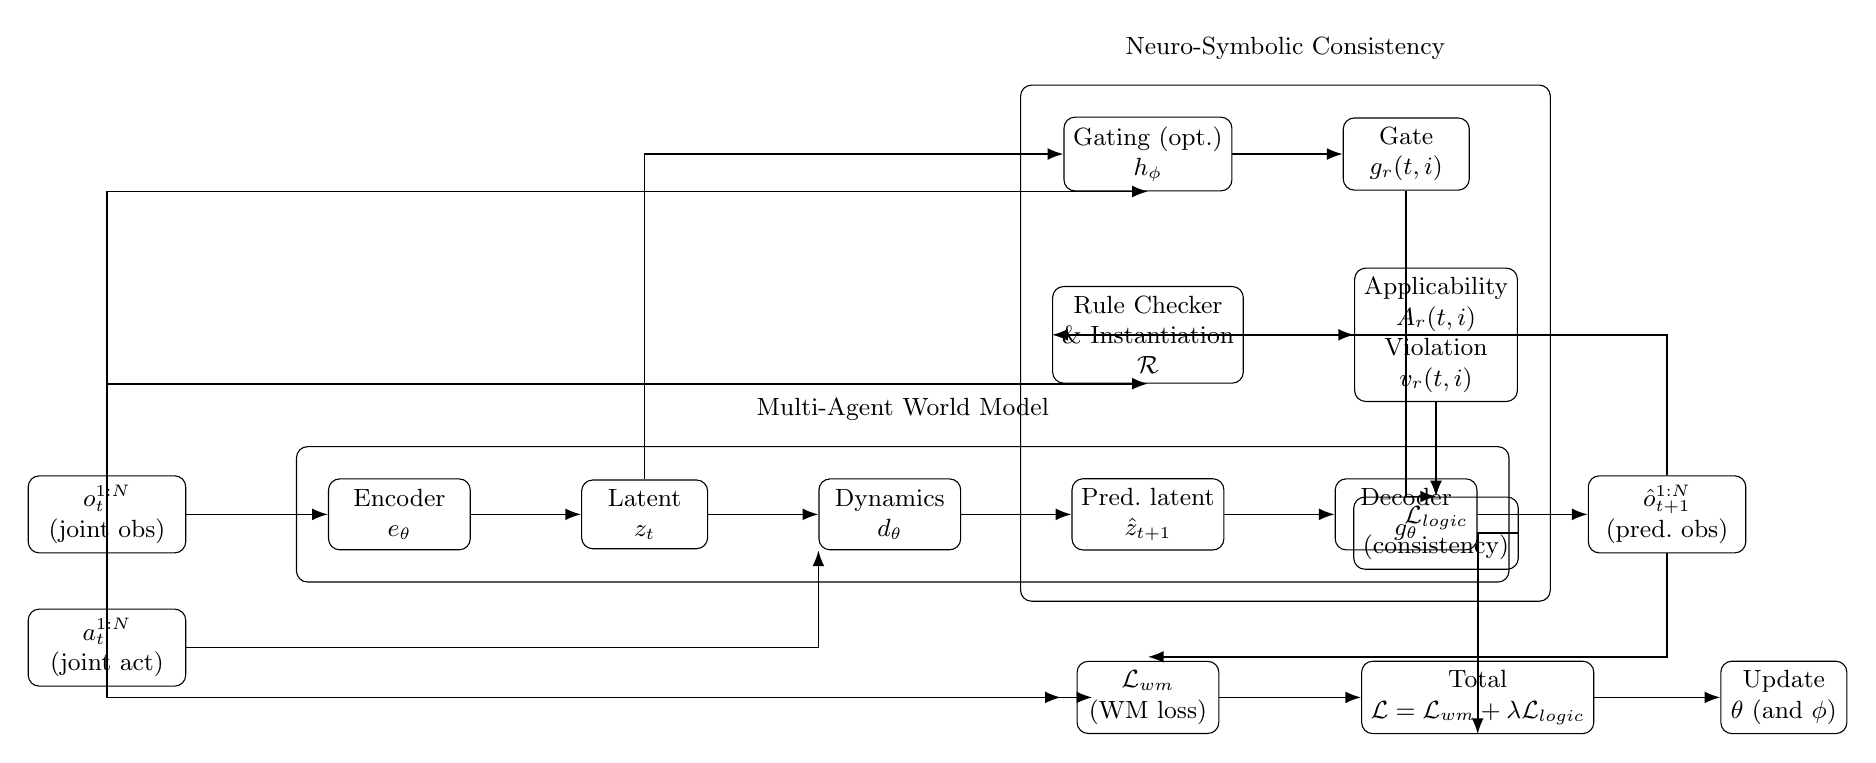
\begin{tikzpicture}[
                font=\small,
                node distance=10mm and 14mm,
                box/.style={draw, rounded corners, align=center, minimum height=9mm, minimum width=18mm},
                smallbox/.style={draw, rounded corners, align=center, minimum height=8mm, minimum width=16mm},
                io/.style={draw, rounded corners, align=center, fill=white, minimum height=8mm, minimum width=20mm},
                loss/.style={draw, rounded corners, align=center, minimum height=9mm, minimum width=18mm},
                group/.style={draw, rounded corners, inner sep=4mm},
                arr/.style={-Latex, line width=0.6pt}
            ]

            % ====== Main WM pipeline ======
            \node[io] (obs) {$o_t^{1:N}$\\(joint obs)};
            \node[io, below=7mm of obs] (act) {$a_t^{1:N}$\\(joint act)};

            \node[box, right=18mm of obs] (enc) {Encoder\\$e_\theta$};
            \node[smallbox, right=14mm of enc] (zt) {Latent\\$z_t$};

            \node[box, right=14mm of zt] (dyn) {Dynamics\\$d_\theta$};
            \node[smallbox, right=14mm of dyn] (znext) {Pred.\ latent\\$\hat z_{t+1}$};

            \node[box, right=14mm of znext] (dec) {Decoder\\$g_\theta$};
            \node[io, right=14mm of dec] (opred) {$\hat o_{t+1}^{1:N}$\\(pred.\ obs)};

            % arrows main
            \draw[arr] (obs) -- (enc);
            \draw[arr] (enc) -- (zt);
            \draw[arr] (zt) -- (dyn);
            \draw[arr] (dyn) -- (znext);
            \draw[arr] (znext) -- (dec);
            \draw[arr] (dec) -- (opred);

            % action into dynamics
            \draw[arr] (act) -| (dyn.south west);

            % ====== Losses ======
            \node[loss, below=14mm of znext] (lwm) {$\mathcal{L}_{wm}$\\(WM loss)};
            \draw[arr] (opred.south) |- ($(lwm.north)+(0,0.5mm)$);
            \draw[arr] (obs.south)  |- ($(lwm.west)+(-2mm,0)$); % indicates supervision / target
            \draw[arr] (act.south)  |- ($(lwm.west)+(2mm,0)$);

            % ====== Neuro-symbolic constraint path ======
            \node[box, above=12mm of znext] (rules) {Rule Checker\\\& Instantiation\\$\mathcal{R}$};
            \node[smallbox, right=14mm of rules] (viol) {Applicability\\$A_r(t,i)$\\Violation\\$v_r(t,i)$};

            \draw[arr] (opred.north) |- (rules.west);
            \draw[arr] (act.north)  |- (rules.south);
            \draw[arr] (rules) -- (viol);

            % gating (optional)
            \node[box, above=12mm of rules] (gate) {Gating (opt.)\\$h_\phi$};
            \node[smallbox, right=14mm of gate] (gcoef) {Gate\\$g_r(t,i)$};

            \draw[arr] (zt.north) |- (gate.west);
            \draw[arr] (act.north) |- (gate.south);
            \draw[arr] (gate) -- (gcoef);

            % logic loss
            \node[loss, below=12mm of viol] (llogic) {$\mathcal{L}_{logic}$\\(consistency)};
            \draw[arr] (viol) -- (llogic);
            \draw[arr] (gcoef) |- (llogic.north);

            % total objective
            \node[loss, right=18mm of lwm] (ltot) {Total\\$\mathcal{L}=\mathcal{L}_{wm}+\lambda\mathcal{L}_{logic}$};
            \draw[arr] (lwm) -- (ltot);
            \draw[arr] (llogic) -| (ltot.south);

            % parameter update annotation
            \node[smallbox, right=16mm of ltot] (upd) {Update\\$\theta$ (and $\phi$)};
            \draw[arr] (ltot) -- (upd);

            % ====== Group boxes (optional, for readability) ======
            \node[group, fit=(enc)(zt)(dyn)(znext)(dec), label={[yshift=2mm]above:Multi-Agent World Model}] (wmgroup) {};
            \node[group, fit=(rules)(viol)(gate)(gcoef)(llogic), label={[yshift=2mm]above:Neuro-Symbolic Consistency}] (nsgroup) {};

        \end{tikzpicture}}

    \caption{Overview of NS-MAWM. A multi-agent world model encodes joint observations, predicts latent dynamics conditioned on joint actions, and decodes predicted observations. Neuro-symbolic rules are instantiated on predictions to compute applicability and violation scores; an optional gating network modulates rule enforcement. Training minimizes $\mathcal{L}_{wm} + \lambda \mathcal{L}_{logic}$.}
    \label{fig:overview}
\end{figure}

  \caption{
  Overview of the NS-MAWM framework.
  Given the joint history $h^j_{t-1}$, joint observation $\omega^j_t$, and joint action $a^j_t$,
  a symbolic transition operator $\mathcal{T}^j_s$ produces determinable features $\omega^{d,j}_{t+1}$
  and a determinability mask $\mathcal{M}_d$, while a neural WM $\mathcal{T}^j_\theta$
  predicts the full next observation.
  Three integration strategies are:
  (\emph{left}) symbolic consistency regularization via an auxiliary loss;
  (\emph{center}) symbolic projection that overwrites neural outputs on determinable features;
  (\emph{right}) residual symbolic dynamics, where symbolic rules predict determinable features
  and the neural model predicts only the remaining ones.
  }
  \label{fig:ns-mawm_overview}
\end{figure}

\subsubsection{Residual symbolic dynamics strategy}
\label{sec:residual_symbolic_dynamics}

Here, we explicitly separate symbolic and symbolic prediction. The neural predictor is trained \emph{only} on features that are not determinable from symbolic knowledge. This architectural partitioning is inspired by residual learning frameworks in neurosymbolic reasoning~\cite{garcez2023neurosymbolic, balloch2023neurosymbolicworldmodelsadapting}. The symbolic model computes:
\begin{align*}
  \omega^{d,j}_{t+1} = \mathcal{T}^j_s(h^j_{t-1}, \omega^j_t, a^j_t),
\end{align*}
while the neural model $\mathcal{T}_{\theta}^{u,j}$ is trained to predict:
\begin{align*}
  \hat{\omega}^{u,j}_{t+1} = \mathcal{T}_{\theta}^{u,j}(h^j_{t-1}, \omega^{u,j}_t, a^j_t).
\end{align*}

The final prediction is assembled by:
\begin{align*}
  \hat{\omega}^{j}_{t+1} = \hat{\omega}^{res,j}_{t+1} = [\omega^{d,j}_{t+1}, \hat{\omega}^{u,j}_{t+1}].
\end{align*}

This strategy reduces model complexity and encourages specialization: symbolic rules govern deterministic patterns, while neural components capture ambiguous or high-entropy transitions. It is particularly advantageous when the symbolic rules cover a stable core of the environment while others remain dynamic.

\subsection{Post-prediction symbolic correction of neural features}
\label{sec:post_prediction_correction}

We introduce a symbolic post-correction mechanism that enforces symbolic consistency
on the neural prediction $\hat{\omega}^j_{t+1}$ at inference time, without retraining via:
%
$\tilde{\omega}^{j}_{t+1} = \mathcal{C}^{s}(\hat{\omega}^{j}_{t+1})$,
%
where $\mathcal{C}^{s}$ applies domain-specific symbolic constraints
(such as mutual exclusivity, valid state transitions, or discretization of categorical features).
This lightweight correction improves semantic coherence and interpretability
of predicted observations.

\subsection{Rule Violation Rate}
\label{sec:rvr}

We quantify symbolic consistency using the \textbf{Rule Violation Rate} (RVR),
which measures how often model predictions violate the symbolic transition rules (\autoref{sec:ns}).

Given the symbolic prediction
$\omega^{d,j}_{t+1} = \mathcal{T}^j_s(h^j_{t-1}, \omega^j_t, a^j_t)$
and the JOPM prediction $\hat{\omega}^j_{t+1}$,
we define the violation indicator:
\begin{equation}
  v_{i,k,t} =
  \begin{cases}
    1 & \text{if } \left| \hat{\omega}^{d}_{i,k,t+1} - \omega^{d}_{i,k,t+1} \right| > \epsilon, \\
    0 & \text{otherwise},
  \end{cases}
\end{equation}
where $(i,k)$ indexes agents and determinable features, and $\epsilon$ is a tolerance threshold.
%
The \textbf{RVR} over $T$ transitions is:
\begin{equation}
  \text{RVR} =
  \frac{1}{n T |\mathcal{F}^d|}
  \sum_{t=1}^T \sum_{i=1}^n \sum_{k \in \mathcal{F}^d} v_{i,k,t}.
\end{equation}

Lower RVR indicates stronger symbolic coherence.
RVR is primarily informative for purely neural WMs
and for symbolic consistency regularization (\autoref{sec:symbolic_loss_regularization});
for symbolic projection and residual symbolic dynamics,
determinable features are enforced by construction and RVR trivially evaluates to zero,
in which case it is mainly used for ablation and diagnostic analysis.


% ============================
% ============================
\section{Evaluation}
\label{sec:eval}

We evaluate NS-MAWM along four axes matching the gaps in \autoref{sec:intro}:
(i) \textbf{long-horizon predictive fidelity} (model bias and compounding errors),
(ii) \textbf{symbolic coherence} (rule satisfaction),
(iii) \textbf{downstream control} (planning / policy performance),
and (iv) \textbf{generalization and robustness} (new configurations and partial rule coverage).

\subsection{Implementation}
\label{sec:impl_overview}

\footnotetext[1]{\label{fn:github}
  An anonymized implementation of NS-MAWM and full experimental details
  (including hyperparameters, architectures, and rule definitions)
  are available at \url{https://anonymous.4open.science/r/NS-MAWM-83D8/README.md}.}

\paragraph{WM backbone.}
Our framework \textit{NS-MAWM}~\hyperref[fn:github]{\footnotemark[1]} builds on a shared MAWM backbone
(\autoref{sec:mawm_basics}) and is implemented in \texttt{PyTorch}~\cite{paszke2019pytorch}.
We use a centralized JOPM comprising
(i) a shared encoder $Enc^j$ over joint observations,
(ii) an LSTM-based latent dynamics core~\cite{hochreiter1997long},
and (iii) a decoder $Dec^j$ predicting the next joint observation.
Joint observations are concatenated along the agent dimension and embedded using MLPs with ReLU activations.
Discrete structured features are one-hot encoded and treated as continuous outputs,
while continuous features are predicted directly.
The prediction loss is
$\mathcal{L}_{\text{pred}} = \sum_{k \in \mathcal{F}_{\text{cont}}}\|\hat{f}_{k}-f_{k}\|^2$.
All neural components are optimized using Adam~\cite{kingma2017adammethodstochasticoptimization}
with a fixed learning rate.

\paragraph{Neuro-symbolic components.}
The symbolic transition operator $\mathcal{T}^j_s$ (\autoref{sec:ns}) is implemented as a lightweight Python rule engine.
Each rule deterministically produces a subset of determinable features $\omega^{d,j}_{t+1}$
and a corresponding mask $\mathcal{M}_d$.
This modular design supports selective rule activation for ablation and robustness studies.
We evaluate three integration strategies (\autoref{sec:strategies}):
(i) symbolic consistency regularization via an auxiliary loss inspired by semantic loss~\cite{Xu2018semanticloss,Fan2017differentiablelearninglogicalrules},
(ii) symbolic projection at inference time,
and (iii) residual symbolic dynamics, restricting neural prediction to non-determinable features.
We further evaluate an inference-time symbolic correction operator $\mathcal{C}^s$
(\autoref{sec:post_prediction_correction}),
which enforces validity constraints (such as mutual exclusivity or spatial feasibility)
using simple projection and discretization operators~\cite{garcez2023neurosymbolic}.

\paragraph{Training data and interfaces.}
WMs are trained offline from replay buffers collected using random or weakly exploratory policies.
We rely on standard MARL interfaces:
\texttt{PettingZoo}~\cite{terry2020pettingzoo},
\texttt{Overcooked-AI}~\cite{Micah2020overcooked},
and the \texttt{SMAC} benchmark~\cite{Ellis2023smacv2}.
Replay buffers store joint observations, actions, and next observations.
To assess data frugality, models are trained on multiple dataset sizes
(such as $N \in \{N_{\text{small}}, N_{\text{med}}, N_{\text{full}}\}$),
while keeping architectures and training schedules fixed across methods.

\paragraph{Hyperparameter selection.}
Neural hyperparameters (learning rate, latent dimension, LSTM size, depth)
are selected automatically using Optuna~\cite{akiba2019optuna}
by minimizing validation prediction loss.
Hyperparameter optimization is applied exclusively to neural components
and independently of symbolic rules, with identical search spaces and budgets across methods.
Selected hyperparameters are fixed for all subsequent experiments.



\subsection{Environments and rule sets}
\label{sec:envs}

We consider four representative multi-agent environments:

\paragraph{(E1) Gridcraft~\hyperref[fn:github-gridcraft]{\footnotemark[2]}, a Minecraft-like gridworld~footnote (discrete, partially observable).}
A grid-based environment with $n$ agents, walls/obstacles, and typed objects.
Observations are structured features (relative positions, occupancy, object presence),
making invariants and equivariances explicit.
Rules~\hyperref[fn:github]{\footnotemark[1]} include collision avoidance, boundary constraints, object persistence, and action-conditioned motion equivariances.

\footnotetext[2]{\label{fn:github-gridcraft}
  An anonymized version is available at: \url{https://anonymous.4open.science/r/Gridcraft-006A/README.md}.}

\paragraph{(E2) Overcooked ~\cite{Micah2020overcooked} (discrete, cooperative coordination).}
We use Overcooked layouts featuring sparse rewards and strong coordination requirements.
Rules~\hyperref[fn:github]{\footnotemark[1]} capture state-transition constraints (pickup/drop interactions), mutually exclusive object states,
and spatial movement constraints.

\paragraph{(E3) Predator--Prey~\cite{lowe2017multi} (continuous or mixed, multi-agent interaction).}
We use a standard Predator--Prey benchmark with continuous positions/velocities (or mixed discrete actions).
Rules~\hyperref[fn:github]{\footnotemark[1]} encode kinematic constraints (bounded velocity), proximity-based capture conditions, and persistence.

\paragraph{(E4) SMAC~\cite{Ellis2023smacv2} (StarCraft Multi-Agent Challenge, partially observable).}
We evaluate on a subset of SMAC scenarios with varying team sizes.
Rules~\hyperref[fn:github]{\footnotemark[1]} focus on movement feasibility and action-conditioned invariances
(such as if an agent does not move, its position remains consistent; cooldown-like constraints).

% \paragraph{Rule sets.}
% For each environment, we define a rule set $\mathcal{R}$~\hyperref[fn:github]{\footnotemark[1]} implementing $\mathcal{T}^j_s$ and the feature mask $\mathcal{M}_d$.
% TODO : donner un aperçu du nombre/type de règles par environnement

\subsection{Computing resources}
\label{sec:resources}

All experiments were conducted on an academic high-performance computing cluster, utilizing various configurations of GPU nodes: we employed nodes equipped with NVIDIA A100 and V100 GPUs, and AMD MI210 GPUs.

% \begin{table*}[!htb]
    \centering
    \footnotesize
    \resizebox{\textwidth}{!}{%
        \begin{tabular}{lcccccccc}
            \toprule
            \multirow{2}{*}{\textbf{Method}}            &
            \multicolumn{2}{c}{\textbf{Gridcraft}}      &
            \multicolumn{2}{c}{\textbf{Overcooked}}     &
            \multicolumn{2}{c}{\textbf{Predator--Prey}} &
            \multicolumn{2}{c}{\textbf{SMAC}}                                                                                                       \\
            \cmidrule(lr){2-3} \cmidrule(lr){4-5} \cmidrule(lr){6-7} \cmidrule(lr){8-9}
                                                        & MSE$_{H}$ $\downarrow$ & RVR $\downarrow$
                                                        & MSE$_{H}$ $\downarrow$ & RVR $\downarrow$
                                                        & MSE$_{H}$ $\downarrow$ & RVR $\downarrow$
                                                        & MSE$_{H}$ $\downarrow$ & RVR $\downarrow$                                                 \\
            \midrule
            MAWM (Neural)                               & 0.092                  & 0.184            & 0.137 & 0.231 & 0.081 & 0.156 & 0.164 & 0.198 \\
            NS-MAWM (Reg.)                              & 0.071                  & 0.061            & 0.101 & 0.084 & 0.067 & 0.052 & 0.131 & 0.073 \\
            NS-MAWM (Projection)                        & 0.068                  & 0.000            & 0.094 & 0.000 & 0.065 & 0.000 & 0.126 & 0.000 \\
            NS-MAWM (Residual)                          & 0.063                  & 0.000            & 0.089 & 0.000 & 0.061 & 0.000 & 0.119 & 0.000 \\
            \bottomrule
        \end{tabular}
    }
    \caption{Quantitative comparison across environments.
        MSE$_H$ denotes multi-step prediction error over open-loop rollouts of horizon $H$.
        RVR is the Rule Violation Rate (\autoref{sec:rvr}).
        Lower is better.}
    \label{tab:results_overview}
\end{table*}



\begin{table*}[!htb]
  \centering
  \footnotesize
  \resizebox{\textwidth}{!}{%
    \begin{tabular}{lcccccccc}
      \toprule
      \multirow{2}{*}{\textbf{Method}}            &
      \multicolumn{2}{c}{\textbf{Gridcraft}}      &
      \multicolumn{2}{c}{\textbf{Overcooked}}     &
      \multicolumn{2}{c}{\textbf{Predator--Prey}} &
      \multicolumn{2}{c}{\textbf{SMAC}}                                                                                                       \\
      \cmidrule(lr){2-3} \cmidrule(lr){4-5} \cmidrule(lr){6-7} \cmidrule(lr){8-9}
                                                  & MSE$_{H}$ $\downarrow$ & RVR $\downarrow$
                                                  & MSE$_{H}$ $\downarrow$ & RVR $\downarrow$
                                                  & MSE$_{H}$ $\downarrow$ & RVR $\downarrow$
                                                  & MSE$_{H}$ $\downarrow$ & RVR $\downarrow$                                                 \\
      \midrule
      MAWM (Neural)                               & 0.094                  & 0.187            & 0.141 & 0.228 & 0.083 & 0.161 & 0.168 & 0.201 \\
      NS-MAWM (Reg.)                              & 0.072                  & 0.064            & 0.106 & 0.089 & 0.069 & 0.055 & 0.134 & 0.076 \\
      NS-MAWM (Projection)                        & 0.067                  & 0.000            & 0.095 & 0.000 & 0.064 & 0.000 & 0.125 & 0.000 \\
      NS-MAWM (Residual)                          & 0.061                  & 0.000            & 0.087 & 0.000 & 0.059 & 0.000 & 0.116 & 0.000 \\
      \bottomrule
    \end{tabular}
  }
  \caption{
    Quantitative evaluation across environments.
    MSE$_H$ denotes the mean squared prediction error aggregated over open-loop rollouts
    of horizon $H$ (lower is better).
    RVR as the rule violation rate (\autoref{sec:rvr}).
    Projection and residual strategies enforce determinable features by construction,
    yielding zero RVR on $\mathcal{F}^d$.
  }
  \label{tab:results_overview}
\end{table*}

\subsection{Evaluation metrics, baselines and protocol}
\label{sec:metrics_baselines_protocol}

\paragraph{Baselines.}
We compare a purely neural multi-agent world model
(\textbf{MAWM (Neural)}) against three NS-MAWM variants:
(i) \textbf{symbolic consistency regularization},
(ii) \textbf{symbolic projection},
and (iii) \textbf{residual symbolic dynamics}.
All methods share the same neural backbone and training budget.
Unless stated otherwise, symbolic post-correction $\mathcal{C}^s$ is disabled.

\paragraph{Predictive fidelity.}
Prediction accuracy is evaluated at one step and over open-loop rollouts
of horizon $H=25$, where model predictions are fed back as inputs.
We report the aggregated multi-step error
$
  \text{MSE}_H =
  \frac{1}{H}
  \sum_{t=1}^{H}
  \mathbb{E}\!\left[
    \|\hat{\omega}^j_t - \omega^j_t\|_2^2
    \right]
$,
averaged over trajectories.

\paragraph{Symbolic coherence.}
Symbolic consistency is measured using the
\textbf{RVR} (\autoref{sec:rvr})
on open-loop rollouts, which quantifies violations of determinable features
$\mathcal{F}^d$.
For projection and residual strategies, determinable features are enforced
by construction, yielding RVR $=0$; RVR therefore primarily diagnoses
the neural baseline and symbolic regularization.

\paragraph{Generalization and robustness.}
Generalization is evaluated on out-of-distribution configurations,
including unseen layouts, varying agent counts,
and alternative SMAC scenarios.
Robustness to incomplete symbolic knowledge is assessed
by randomly dropping a fraction $\rho \in \{0.25, 0.5\}$
of symbolic rules during training and inference.

\paragraph{Protocol.}
For each environment, all methods are trained on the same offline dataset
and identical train/validation splits, and evaluated on held-out trajectories.
Results are reported as mean $\pm$ standard error over 5 random seeds.

\subsection{Results}
\label{sec:results}

\autoref{tab:results_overview} reports quantitative results
across all environments and evaluation dimensions.

\paragraph{Long-horizon prediction accuracy and error accumulation (G1).}
Across all environments, NS-MAWM variants
consistently improve long-horizon predictive fidelity
over the purely neural MAWM baseline.
In simpler settings such as Gridcraft,
the baseline already achieves low error (MSE$_H = 0.094$),
yet neuro-symbolic integration further reduces compounding error,
with the residual strategy reaching MSE$_H = 0.061$
($\approx 35\%$ relative improvement).

The benefits become more pronounced
as dynamics grow more constrained and interaction-heavy.
In Overcooked and SMAC,
where small inconsistencies rapidly cascade during open-loop rollouts,
the neural MAWM exhibits substantially higher error
(MSE$_H = 0.141$ and $0.168$).
Here, NS-MAWM achieves larger gains,
with the residual strategy reducing MSE$_H$
by $38\%$ and $31\%$, respectively.
These results indicate that symbolic constraints
act as inductive biases
that effectively limit long-horizon semantic drift.

\paragraph{Symbolic coherence and constraint satisfaction (G2, G3).}
The RVR highlights a clear gap
between numerical accuracy and semantic validity
in purely neural world models.
Despite moderate MSE$_H$,
the MAWM baseline violates symbolic constraints
in $16\%$ to $23\%$ of determinable features,
showing that likelihood-based objectives alone
do not enforce logical or physical consistency.

Symbolic consistency regularization
reduces RVR by roughly a factor of three across environments
(from $0.228$ to $0.089$ in Overcooked),
but residual violations remain.
In contrast, symbolic projection and residual symbolic dynamics
enforce determinable features by construction,
yielding zero RVR in all settings.
This hard enforcement eliminates an entire class
of semantically invalid predictions,
demonstrating that symbolic coherence
must be explicitly optimized rather than treated as emergent.

\paragraph{Comparing integration strategies.}
While all NS-MAWM variants outperform the neural baseline,
clear differences emerge between integration strategies.
Symbolic regularization provides consistent improvements
with minimal architectural changes,
but remains sensitive to residual violations.
Symbolic projection guarantees perfect rule satisfaction
on determinable features,
while still relying on neural prediction elsewhere.

Residual symbolic dynamics achieves the strongest overall trade-off.
By assigning deterministic components to symbolic transitions
and restricting neural learning to undeterminable features,
it simultaneously attains the lowest MSE$_H$
and zero RVR across all environments.
This separation reduces model complexity,
limits error accumulation,
and improves stability over long rollouts,
making residual symbolic dynamics
particularly well suited for structured multi-agent settings.

\section{Conclusion and future work}
\label{sec:conclusion}

We proposed \textbf{NS-MAWM}, a neuro-symbolic framework for MAWM that integrates symbolic reasoning. By enforcing symbolic coherence, NS-MAWM reduces long-horizon semantic drift and improves imagination-based planning, yielding consistent gains in predictive fidelity and generalization over purely neural WMs.

Despite its benefits, NS-MAWM incurs additional computational overhead,
faces scalability challenges as the number of agents, features, or symbolic rules grows,
and relies on handcrafted symbolic rules.
Future work will explore:
(1) leveraging Large Language Models~\cite{Brown2020gpt3,openai2023gpt4} to assist in automatic rule extraction or refinement;
(2) developing matrix-oriented formulations of symbolic transitions to reduce overhead and improve scalability;
and (3) adopting high-performance numerical frameworks such as \texttt{JAX}~\cite{jax2018github}
to enable efficient vectorization, compilation, and hardware acceleration.


\section*{Impact Statement}

This paper presents work whose goal is to advance the field of Machine Learning by improving the reliability of model-based multi-agent reinforcement learning.
By reducing semantic inconsistencies in learned WMs, this work may contribute to safer and more interpretable decision-making in multi-agent systems.
We do not identify ethical concerns specific to this work beyond those commonly associated with reinforcement learning research.


% ============================
% Acknowledgements (remove for submission if needed)
% ============================
% \section*{Acknowledgements}

% ============================
% References
% ============================
\bibliography{references}
\bibliographystyle{icml2026}

%%%%%%%%%%%%%%%%%%%%%%%%%%%%%%%%%%%%%%%%%%%%%%%%%%%%%%%%%%%%%%%%%%%%%%%%%%%%%%%
%%%%%%%%%%%%%%%%%%%%%%%%%%%%%%%%%%%%%%%%%%%%%%%%%%%%%%%%%%%%%%%%%%%%%%%%%%%%%%%
% APPENDIX
%%%%%%%%%%%%%%%%%%%%%%%%%%%%%%%%%%%%%%%%%%%%%%%%%%%%%%%%%%%%%%%%%%%%%%%%%%%%%%%
%%%%%%%%%%%%%%%%%%%%%%%%%%%%%%%%%%%%%%%%%%%%%%%%%%%%%%%%%%%%%%%%%%%%%%%%%%%%%%%

\newpage

% \appendix

% \section{Rule Set Details}
% \label{app:rules}
% % TODO:
% % - list rules formally
% % - applicability masks
% % - examples

% \section{Additional Experimental Results}
% \label{app:more}
% % TODO:
% % - ablations, extra environments, hyperparams

% \section{Architectures and Hyperparameters}
% \label{app:hparams}
% % TODO:
% % - full hyperparam tables

%%%%%%%%%%%%%%%%%%%%%%%%%%%%%%%%%%%%%%%%%%%%%%%%%%%%%%%%%%%%%%%%%%%%%%%%%%%%%%%
%%%%%%%%%%%%%%%%%%%%%%%%%%%%%%%%%%%%%%%%%%%%%%%%%%%%%%%%%%%%%%%%%%%%%%%%%%%%%%%

\end{document}
